\chapter{Ondas em cordas e barras: a equação de d'Alembert}\label{ch:b2:waves-on-strings}

Belisque a corda de um violão e uma forma corre por ela, bate no
cavalete, volta e se acomoda no padrão estacionário cuja
frequência você ouve como uma nota. Encoste o ouvido num trilho e
você ouve o trem muito antes de ele chegar: uma compressão desce pelo
aço a cinco quilômetros por segundo. O volume do Ano 1 descreveu essas
ondas --- progressivas, estacionárias, superpostas --- sem dizer por que
existem. Este capítulo deduz a equação que as governa, a
\emph{\omterm{thm:b2:waves-on-strings:equation}{equação de onda} de d'Alembert}, primeiro para o movimento transversal de uma
corda, depois para o movimento longitudinal de uma barra construída, átomo a átomo,
de massas e molas; ele calcula a energia que uma onda transporta e a
impedância que decide o que acontece quando ela encontra uma mudança de meio.

\section{A corda vibrante}

\begin{theorem}[Equação de onda de uma corda]\label{thm:b2:waves-on-strings:equation}
\index{equação de d'Alembert}\index{equação de onda}\index{celeridade das ondas (corda)}
Uma corda de massa linear $\mu$, esticada com tração $T$, faz
pequenos deslocamentos transversais $y(x, t)$ (inclinações $|\partial_xy| \ll 1$). Então
\[
\frac{\partial^2y}{\partial t^2} = c^2\,\frac{\partial^2y}{\partial x^2} ,
\qquad c = \sqrt{\frac{T}{\mu}} ,
\]
a \emph{\omterm{thm:b2:waves-on-strings:equation}{equação de d'Alembert}}, cuja solução geral é $y = f(x - ct)
+ g(x + ct)$: a superposição de uma forma que viaja para a direita e
outra que viaja para a esquerda com celeridade $c$, sem se deformar.
\end{theorem}

\begin{proof}
Isole o elemento entre $x$ e $x + \dd x$, de massa $\mu\,\dd x$. Seus
vizinhos o puxam ao longo da tangente à corda com a tração $T$:
horizontalmente $T\cos\theta \approx T$ nas duas pontas (não há movimento horizontal, de modo que
$T$ é a mesma ao longo de tudo), verticalmente $T\sin\theta \approx T\partial_xy$, o que
dá a força resultante $T[\partial_xy(x + \dd x) - \partial_xy(x)] = T\,\partial_x^2y\,\dd x$.
Newton: $\mu\,\dd x\,\partial_t^2y = T\partial_x^2y\,\dd x$. Para a solução, ponha
$u = x - ct$, $v = x + ct$: a equação torna-se $\partial_u\partial_vy = 0$
(regra da cadeia), de modo que $\partial_vy$ só depende de $v$, e $y = f(u) + g(v)$;
reciprocamente, todo $y$ dessa forma a satisfaz. A gravidade, desprezada, é legítima
quando $T \gg \mu gL$.
\end{proof}

\begin{omfigure}
\begin{tikzpicture}[font=\small, x=1cm, y=1cm, >=Stealth]
  \begin{scope}
    \draw[->] (-2.5,0) -- (3.0,0) node[right, font=\footnotesize] {$x$};
    \draw[omDef, very thick, domain=-2.3:2.8, samples=60] plot (\x,{0.9*exp(-(\x)^2/1.6)});
    \coordinate (A) at (-0.6,{0.9*exp(-0.36/1.6)}); \coordinate (B) at (0.2,{0.9*exp(-0.04/1.6)});
    \fill[omThm] (A) circle (1.5pt); \fill[omThm] (B) circle (1.5pt);
    \draw[omThm, very thick, ->] (A) -- ($(A)+(-0.9,-0.55)$) node[above left, font=\footnotesize, yshift=2pt] {$\vect T(x)$};
    \draw[omThm, very thick, ->] (B) -- ($(B)+(1.0,-0.12)$) node[right, font=\footnotesize] {$\vect T(x+\dd x)$};
    \draw[dashed] (-0.6,0) -- (A); \draw[dashed] (0.2,0) -- (B);
    \node[font=\footnotesize] at (-0.6,-0.3) {$x$}; \node[font=\footnotesize] at (0.35,-0.3) {$x + \dd x$};
    \node[font=\footnotesize] at (0.2,-0.9) {$\mu\,\dd x\,\partial_t^2y = T\,\partial_x^2y\,\dd x$};
  \end{scope}
  \begin{scope}[xshift=7.6cm]
    \draw[->] (-2.5,0) -- (3.0,0) node[right, font=\footnotesize] {$x$};
    \draw[omDef, thick, domain=-2.3:2.8, samples=60] plot (\x,{0.8*exp(-(\x+1.3)^2/0.5)});
    \draw[omDef, thick, dashed, domain=-2.3:2.8, samples=60] plot (\x,{0.8*exp(-(\x-0.5)^2/0.5)});
    \draw[omDef, thick, ->] (-1.0,1.0) -- (0.2,1.0) node[above, font=\footnotesize, pos=0.5] {$c$};
    \node[font=\footnotesize] at (-1.3,-0.35) {$t$}; \node[font=\footnotesize] at (0.5,-0.35) {$t + \tau$};
    \node[font=\footnotesize] at (0.2,-0.9) {$y = f(x - ct)$};
  \end{scope}
\end{tikzpicture}

{\small À esquerda: as forças sobre um elemento de corda --- as duas trações
não são paralelas quando a corda está curvada, e sua resultante é
transversal. À direita: uma forma $f(x - ct)$ viaja para a direita a $c$
sem se deformar.}
\end{omfigure}

\begin{example}[Violão, piano, cabo]\label{ex:b2:waves-on-strings:numbers}
A corda mi grave de um violão ($\mu = \qty{5.5}{g/m}$, comprimento \qty{0.65}{m},
\qty{82.4}{Hz}) vibra em seu fundamental com $\lambda = 2L$: $c = 2Lf =
\qty{107}{m/s}$ e $T = \mu c^2 = \qty{63}{N}$. A corda lá$_4$ de um piano (aço,
\qty{1}{mm}, $\mu = \qty{6.1}{g/m}$, \qty{0.38}{m}, \qty{440}{Hz}): $c = \qty{334}{m/s}$,
$T = \qty{680}{N}$ --- e há cerca de $230$ cordas num piano, vinte
toneladas de tração sobre uma placa de ferro fundido. Um cabo de \qty{1}{kg/m} a \qty{10}{kN}:
\qty{100}{m/s}.
\end{example}

\section{Ondas estacionárias e modos}

\begin{proposition}[Modos de uma corda fixa nas duas pontas]\label{prop:b2:waves-on-strings:modes}
\index{modos próprios}\index{harmônicos}\index{onda estacionária}
Uma corda fixa em $x = 0$ e $x = L$ admite as soluções senoidais
estacionárias (\emph{\omterm{prop:b2:waves-on-strings:modes}{modos próprios}})
\[
y_n(x, t) = A_n\sin\frac{n\pi x}{L}\cos(\omega_nt - \varphi_n) , \qquad
f_n = \frac{\omega_n}{2\pi} = n\,\frac{c}{2L} = n f_1 , \quad n = 1, 2, 3, \dots
\]
--- o fundamental $f_1 = c/2L$ e seus \emph{harmônicos}. O modo $n$ tem
$n - 1$ nós entre as extremidades. Todo movimento da corda é uma
superposição $y = \sum_ny_n$, com as amplitudes e as fases fixadas
pela forma e pela velocidade iniciais (uma série de Fourier, como o volume
de matemática deste ano estabelece): a mistura de harmônicos é o
\emph{timbre} da nota.
\end{proposition}

\begin{proof}
Procure $y = F(x)\cos(\omega t - \varphi)$: $F'' + (\omega/c)^2F = 0$, e $F(0) = 0$ dá
$F = A\sin(\omega x/c)$, enquanto $F(L) = 0$ exige $\omega L/c = n\pi$. Cada modo é
também a soma de duas ondas progressivas: $\sin kx\cos\omega t = \tfrac12[\sin(kx -
\omega t) + \sin(kx + \omega t)]$ --- a onda e sua reflexão. A
completude dos senos é o teorema de Fourier.
\end{proof}

\begin{omfigure}
\begin{tikzpicture}
\begin{axis}[omaxis, axis x line=bottom, axis y line=none, width=6.4cm, height=5.2cm,
    xmin=0, xmax=1, ymin=-5.9, ymax=1.5, xtick={0,1}, xticklabels={$0$, $L$}, samples=80,
    xlabel={}, ylabel={}]
  \addplot[omDef, thick, domain=0:1] {sin(deg(pi*x))};
  \addplot[omDef, thick, dashed, domain=0:1] {-sin(deg(pi*x))};
  \addplot[omThm, thick, domain=0:1] {0.8*sin(deg(2*pi*x))-2.6};
  \addplot[omThm, thick, dashed, domain=0:1] {-0.8*sin(deg(2*pi*x))-2.6};
  \addplot[omProp, thick, domain=0:1] {0.7*sin(deg(3*pi*x))-5.0};
  \addplot[omProp, thick, dashed, domain=0:1] {-0.7*sin(deg(3*pi*x))-5.0};
  \addplot[black, thin] coordinates {(0,-2.6) (1,-2.6)};
  \addplot[black, thin] coordinates {(0,-5.0) (1,-5.0)};
  \node[font=\scriptsize] at (axis cs:0.5,1.25) {$n = 1$};
  \node[font=\scriptsize] at (axis cs:0.5,-1.4) {$n = 2$};
  \node[font=\scriptsize] at (axis cs:0.5,-3.85) {$n = 3$};
\end{axis}
\end{tikzpicture}
\hfill
\begin{tikzpicture}
\begin{axis}[omaxis, axis x line=bottom, axis y line=left, width=5.0cm, height=4.2cm,
    xlabel={$x/L$}, ylabel={$y$}, xmin=0, xmax=1, ymin=-0.05, ymax=1.1, xtick={0,0.5,1}, ytick=\empty, samples=200, clip=false,
    xlabel style={at={(axis description cs:0.5,-0.12)}, anchor=north},
    ylabel style={at={(axis description cs:-0.06,0.5)}, rotate=90, anchor=south}]
  \addplot[black, thick] coordinates {(0,0) (0.5,1) (1,0)};
  \addplot[omDef, thick, domain=0:1] {0.81*sin(deg(pi*x))};
  \addplot[omThm, thick, domain=0:1] {0.81*sin(deg(pi*x)) - 0.09*sin(deg(3*pi*x))};
  \node[font=\scriptsize, anchor=west] at (axis cs:0.03,0.95) {pinçada};
  \node[font=\scriptsize, omDef, anchor=east] at (axis cs:0.97,0.95) {$n = 1$};
  \node[font=\scriptsize, omThm, anchor=east] at (axis cs:0.97,0.78) {$n = 1, 3$};
\end{axis}
\end{tikzpicture}

{\small À esquerda: os três primeiros modos de uma corda fixa nas duas pontas ($f_n = nc/2L$).
À direita: uma corda pinçada no meio (triângulo) e os primeiros termos
de sua série de Fourier --- só aparecem harmônicos ímpares, com amplitudes
que caem como $1/n^2$.}
\end{omfigure}

\begin{example}[A experiência de Melde]\label{ex:b2:waves-on-strings:melde}
\index{experiência de Melde}
Uma corda excitada numa ponta por um vibrador de frequência $f$, com a outra ponta
passando por uma polia até uma massa $m$ pendurada (de modo que $T = mg$): uma grande
\omterm{prop:b2:waves-on-strings:modes}{onda estacionária} aparece sempre que $f$ é igual a um dos $f_n = (n/2L)
\sqrt{mg/\mu}$ --- ressonância do modo $n$. Para $L = \qty{1.2}{m}$, $\mu =
\qty{1.0}{g/m}$ e $f = \qty{50}{Hz}$, as massas que dão $n = 1, 2, 3$ ventres
são $m_n = 4L^2f^2\mu/n^2g = 1.47/n^2$ kg: \qty{1.47}{kg}, \qty{367}{g}, \qty{163}{g}.
Apertar a corda de um violão no décimo segundo traste reduz $L$ à metade e dobra
$f_1$: a oitava; tocá-la de leve no meio, sem apertar,
mata os modos ímpares e deixa o segundo harmônico --- o harmônico natural.
\end{example}

\section{Energia, potência e impedância}

\begin{proposition}[Energia de uma onda numa corda]\label{prop:b2:waves-on-strings:energy}
\index{densidade de energia (corda)}\index{fluxo de energia (corda)}\index{impedância (corda)}
Uma corda transporta a energia por unidade de comprimento e a potência (fluxo
de energia no sentido $+x$)
\[
e = \tfrac12\mu\Bigl(\frac{\partial y}{\partial t}\Bigr)^2 + \tfrac12T\Bigl(\frac{\partial y}{\partial x}\Bigr)^2 ,
\qquad
\mathcal P = -T\,\frac{\partial y}{\partial x}\,\frac{\partial y}{\partial t} ,
\]
que obedecem ao balanço local $\partial_te + \partial_x\mathcal P = 0$. Para uma
onda progressiva $y = f(x - ct)$, as densidades cinética e potencial são
iguais e $\mathcal P = Z\,(\partial_ty)^2$ com
\[
Z = \sqrt{T\mu} = \mu c = \frac Tc ,
\]
a \emph{impedância} da corda (\unit{kg/s}): a razão entre a força
transversal $-T\partial_xy$ exercida pela corda sobre o que está adiante
e a velocidade transversal $\partial_ty$. Uma onda senoidal de amplitude $A$
transporta a potência média $\langle\mathcal P\rangle = \tfrac12Z\omega^2A^2$.
\end{proposition}

\begin{proof}
O termo potencial é o trabalho da tração ao esticar o elemento:
seu comprimento vale
\[
\dd x\sqrt{1 + (\partial_xy)^2} \approx \dd x\bigl(1 + \tfrac12(\partial_xy)^2\bigr) ,
\]
de modo que o excesso de comprimento vezes $T$ dá $\tfrac12T(\partial_xy)^2\dd x$. A potência
transmitida através de $x$ no sentido $+x$ é a força transversal exercida
pela parte esquerda sobre a direita, $-T\partial_xy$, vezes a velocidade
$\partial_ty$. Balanço:
\[
\partial_te = \mu\,\partial_ty\,\partial_t^2y + T\,\partial_xy\,\partial_x\partial_ty ,
\qquad
-\partial_x\mathcal P = T\,\partial_x^2y\,\partial_ty + T\,\partial_xy\,\partial_x\partial_ty ,
\]
iguais pela \omterm{thm:b2:waves-on-strings:equation}{equação de onda}. Para $f(x - ct)$: $\partial_xy = -\partial_ty/c$, logo $\mathcal P = (T/c)
(\partial_ty)^2$ e as duas densidades valem $\tfrac12\mu(\partial_ty)^2$.
\end{proof}

\begin{proposition}[Reflexão e transmissão numa junção]\label{prop:b2:waves-on-strings:junction}
\index{coeficiente de reflexão (corda)}\index{coeficiente de transmissão (corda)}
Uma onda de amplitude $A_i$ chega, vinda de uma corda de impedância $Z_1$, a
uma corda de impedância $Z_2$ unida a ela em $x = 0$. A continuidade do
deslocamento e da força transversal na junção dá os
coeficientes de amplitude
\[
r = \frac{A_r}{A_i} = \frac{Z_1 - Z_2}{Z_1 + Z_2} , \qquad
t = \frac{A_t}{A_i} = \frac{2Z_1}{Z_1 + Z_2} ,
\]
e as frações de energia $R = r^2$, $\mathcal T = 4Z_1Z_2/(Z_1 + Z_2)^2$, com
$R + \mathcal T = 1$. Uma extremidade fixa ($Z_2 \to \infty$) reflete com $r = -1$
(o pulso volta invertido), uma extremidade livre ($Z_2 = 0$) com $r = +1$;
impedâncias iguais transmitem tudo.
\end{proposition}

\begin{proof}
Ondas senoidais $y_1 = A_i\cos(\omega t - k_1x) + A_r\cos(\omega t + k_1x)$ para
$x < 0$, $y_2 = A_t\cos(\omega t - k_2x)$ para $x > 0$, com o mesmo $\omega$ dos dois
lados. Em $x = 0$: $y_1 = y_2$ dá $A_i + A_r = A_t$; a força $-T\partial_xy$
contínua (junção sem massa) dá $Z_1(A_i - A_r) = Z_2A_t$ (usando
$T_1k_1 = Z_1\omega$). Resolva. Energias: as potências médias $\tfrac12Z\omega^2A^2$.
\end{proof}

\begin{omfigure}
\begin{tikzpicture}[font=\small, x=1cm, y=1cm, >=Stealth]
  \begin{scope}
    \draw[->] (-3.2,0) -- (3.2,0) node[right, font=\footnotesize] {$x$};
    \draw[omDef, very thick, domain=-3.0:0, samples=50] plot (\x,{0.8*exp(-(\x+1.6)^2/0.25)});
    \draw[omDef, very thick, domain=0:3.0, samples=50] plot (\x,{0});
    \fill (0,0) circle (2pt); \node[font=\footnotesize] at (0,-0.35) {$Z_1 \to Z_2$};
    \draw[omDef, ->, thick] (-1.6,1.0) -- (-0.8,1.0) node[above, font=\footnotesize, pos=0.5] {$A_i$};
    \node[font=\footnotesize] at (-1.5,-0.6) {$Z_1$}; \node[font=\footnotesize] at (1.5,-0.6) {$Z_2 > Z_1$};
    \node[font=\footnotesize] at (0,-1.1) {antes};
  \end{scope}
  \begin{scope}[xshift=7.2cm]
    \draw[->] (-3.2,0) -- (3.2,0) node[right, font=\footnotesize] {$x$};
    \draw[omThm, very thick, domain=-3.0:0, samples=50] plot (\x,{-0.27*exp(-(\x+1.6)^2/0.25)});
    \draw[omProp, very thick, domain=0:3.0, samples=50] plot (\x,{0.53*exp(-(\x-1.1)^2/0.12)});
    \fill (0,0) circle (2pt);
    \draw[omThm, ->, thick] (-1.0,0.5) -- (-1.8,0.5) node[above, font=\footnotesize, pos=0.5] {$rA_i$};
    \draw[omProp, ->, thick] (1.0,0.9) -- (1.8,0.9) node[above, font=\footnotesize, pos=0.5] {$tA_i$};
    \node[font=\footnotesize] at (0,-1.1) {depois: $r = \dfrac{Z_1 - Z_2}{Z_1 + Z_2}$, $t = \dfrac{2Z_1}{Z_1 + Z_2}$};
  \end{scope}
\end{tikzpicture}

{\small Um pulso encontra uma junção com uma corda mais pesada ($Z_2 = 4Z_1$):
uma parte é transmitida, mais lenta e mais estreita, outra é refletida invertida.}
\end{omfigure}

\section{Da cadeia de átomos à barra elástica}

\begin{proposition}[A cadeia de átomos; o módulo de Young]\label{prop:b2:waves-on-strings:chain}
\index{cadeia de átomos}\index{módulo de Young}\index{lei de Hooke}\index{onda longitudinal}
Uma fila de massas idênticas $m$ separadas por $a$ e ligadas por molas de
rigidez $k$: se $u_n(t)$ é o deslocamento da massa $n$ ao longo da
fila,
\[
m\ddot u_n = k(u_{n+1} - u_n) - k(u_n - u_{n-1}) = k(u_{n+1} - 2u_n + u_{n-1}) .
\]
Quando o deslocamento varia lentamente de uma massa à seguinte (em
comprimentos de onda $\lambda \gg a$), $u_n(t) \to u(x, t)$ com $u_{n\pm1} - u_n \approx
\pm a\,\partial_xu + \tfrac12a^2\partial_x^2u$, e a cadeia obedece à \omterm{thm:b2:waves-on-strings:equation}{equação de
d'Alembert}
\[
\frac{\partial^2u}{\partial t^2} = c^2\frac{\partial^2u}{\partial x^2} , \qquad
c = a\sqrt{\frac km} = \sqrt{\frac{E}{\rho}} ,
\]
com $\rho = m/a^3$ a massa específica de um sólido feito dessas cadeias num
arranjo cúbico e $E = k/a$ seu \emph{\omterm{prop:b2:waves-on-strings:chain}{módulo de Young}}: a rigidez de
uma barra de seção $S$ e comprimento $\ell$ vale $kS/a^2\cdot a/\ell = ES/\ell$,
ou seja, a \emph{\omterm{prop:b2:waves-on-strings:chain}{lei de Hooke}} $F/S = E\,\Delta\ell/\ell$ (tensão $\sigma = E\varepsilon$).
\end{proposition}

\begin{proof}
Cada mola é esticada pela diferença dos deslocamentos de suas
pontas. Insira as expansões de Taylor: $m\partial_t^2u = ka^2\partial_x^2u$. Um cubo de
lado $a$ por átomo dá $\rho = m/a^3$; uma barra de seção $S$ contém
$S/a^2$ cadeias paralelas de $\ell/a$ molas em série, de rigidez total
$(S/a^2)(ka/\ell) = (k/a)S/\ell$.
\end{proof}

\begin{proposition}[Ondas longitudinais numa barra]\label{prop:b2:waves-on-strings:rod}
\index{som nos sólidos}
Diretamente no contínuo: um elemento de barra entre $x$ e $x +
\dd x$, deslocado de $u(x, t)$, sofre a deformação $\varepsilon = \partial_xu$ e é puxado
pela tensão $\sigma = E\partial_xu$ em cada face; Newton dá $\rho\,\partial_t^2u =
E\,\partial_x^2u$: as \omterm{prop:b2:waves-on-strings:chain}{ondas longitudinais} (de compressão) viajam a $c = \sqrt{E/\rho}$
--- \qty{5100}{m/s} no aço ($E = \qty{200}{GPa}$), \qty{5000}{m/s} no alumínio,
\qty{3700}{m/s} no granito, \qty{3500}{m/s} na madeira ao longo das fibras. A
impedância vale $Z = \rho c = \sqrt{E\rho}$ por unidade de área, e as mesmas
fórmulas de junção se aplicam --- é assim que o ultrassom encontra uma trinca num
trilho.
\end{proposition}

\begin{proof}
Força resultante sobre o elemento: $S[\sigma(x + \dd x) - \sigma(x)] = SE\partial_x^2u\,\dd x$;
massa $\rho S\dd x$.
\end{proof}

\begin{omfigure}
\begin{tikzpicture}[font=\small, x=1cm, y=1cm, >=Stealth]
  \begin{scope}
    \foreach \i in {0,1,2,3,4} {
      \fill[omDef] ({1.4*\i},0) circle (5pt);
    }
    \foreach \i in {0,1,2,3} {
      \draw[thick, decorate, decoration={coil, aspect=0.5, segment length=4pt, amplitude=3pt}] ({1.4*\i+0.18},0) -- ({1.4*\i+1.22},0);
    }
    \node[font=\footnotesize] at (1.4,-0.5) {$u_{n-1}$}; \node[font=\footnotesize] at (2.8,-0.5) {$u_n$}; \node[font=\footnotesize] at (4.2,-0.5) {$u_{n+1}$};
    \draw[<->] (1.4,0.45) -- (2.8,0.45) node[midway, above, font=\footnotesize] {$a$};
    \node[font=\footnotesize] at (2.8,-1.1) {$m\ddot u_n = k(u_{n+1} - 2u_n + u_{n-1})$};
  \end{scope}
  \begin{scope}[xshift=8.0cm]
    \draw[thick] (-2.0,-0.5) rectangle (2.6,0.5);
    \fill[omDef!25] (-0.3,-0.5) rectangle (0.5,0.5);
    \draw[omThm, very thick, ->] (-0.3,0) -- (-1.2,0) node[above, font=\footnotesize, pos=0.6] {$\sigma(x)S$};
    \draw[omThm, very thick, ->] (0.5,0) -- (1.5,0) node[above, font=\footnotesize, pos=0.6] {$\sigma(x + \dd x)S$};
    \node[font=\footnotesize] at (0.1,-0.8) {$\rho S\dd x\,\partial_t^2u = SE\,\partial_x^2u\,\dd x$};
    \node[font=\footnotesize] at (0.3,-1.35) {$c = \sqrt{E/\rho}$};
  \end{scope}
\end{tikzpicture}

{\small À esquerda: a cadeia de massas e molas --- cada massa sente as
duas molas que a cercam, e o limite contínuo é a \omterm{thm:b2:waves-on-strings:equation}{equação de onda}
com $c = a\sqrt{k/m}$. À direita: um elemento de barra elástica puxado pela
tensão em suas duas faces.}
\end{omfigure}

\begin{remark}[O que a cadeia sabe e a barra não]\label{rem:b2:waves-on-strings:dispersion}
Procurar $u_n = A\cos(\omega t - kna)$ na equação exata da cadeia dá
$\omega = 2\sqrt{k/m}\,|\sin(ka/2)|$: para $ka \ll 1$ isso é $\omega = ck$, a
\omterm{thm:b2:waves-on-strings:equation}{equação de onda} não dispersiva, mas quando o comprimento de onda se aproxima de $2a$ a
frequência satura em $2\sqrt{k/m}$ e as velocidades de fase e de grupo
diferem --- a primeira \emph{relação de dispersão} deste volume, o
assunto do \cref{ch:b2:dispersion-wave-packets}. Para $a = \qty{0.25}{nm}$ e
$c = \qty{5}{km/s}$ o corte fica em $\omega_{\max} = 2c/a = \qty{4e13}{rad/s}$
(\qty{6}{THz}): o sólido não pode vibrar mais rápido do que as molas de seus átomos
permitem.
\end{remark}

\section{Exercícios}

\begin{exercise}[$\star$]\label{exo:b2:waves-on-strings:1}
A corda lá de um violão (\qty{110}{Hz}, $L = \qty{65}{cm}$, $\mu = \qty{3.0}{g/m}$):
celeridade das ondas, tração, comprimento de onda do fundamental na corda e
do som no ar; frequência quando a corda é apertada no quinto
traste ($L$ reduzido por um fator $2^{-5/12}$).
\end{exercise}

\begin{exercise}[$\star$]\label{exo:b2:waves-on-strings:2}
Celeridade das \omterm{prop:b2:waves-on-strings:chain}{ondas longitudinais} no aço ($E = \qty{200}{GPa}$, $\rho =
\qty{7800}{kg/m^3}$), no alumínio (\qty{70}{GPa}, \qty{2700}{kg/m^3}) e no chumbo
(\qty{16}{GPa}, \qty{11300}{kg/m^3}). Tempo que um som leva para percorrer \qty{1.0}{km}
por um trilho e pelo ar (\qty{340}{m/s}); o que ouve quem encosta o
ouvido no trilho.
\end{exercise}

\begin{exercise}[$\star$]\label{exo:b2:waves-on-strings:3}
Uma corda de fundamental \qty{200}{Hz}: frequências e número de nós dos
modos 2, 3 e 4; posições dos nós do modo 3; frequência do
fundamental se a tração dobra, se o comprimento cai à metade, se a
corda é trocada por outra três vezes mais pesada por metro.
\end{exercise}

\begin{exercise}[$\star$]\label{exo:b2:waves-on-strings:4}
Uma corda de \qty{12}{m} ($\mu = \qty{0.20}{kg/m}$) é tracionada com \qty{45}{N}; uma
ponta está presa a uma parede. Um pulso é enviado da outra ponta. Celeridade;
tempo para chegar à parede e voltar; forma do pulso que volta;
o mesmo se a ponta distante estiver amarrada a um anel leve que desliza livremente num
mastro.
\end{exercise}

\begin{exercise}[$\star\star$]\label{exo:b2:waves-on-strings:5}
Uma corda de piano para \qty{440}{Hz}: aço ($\rho = \qty{7800}{kg/m^3}$),
diâmetro \qty{1.0}{mm}, comprimento vibrante \qty{38}{cm}. (a) $\mu$, celeridade das ondas,
tração. (b) Tensão no fio; compare com a resistência do fio de
piano, cerca de \qty{2}{GPa}. (c) A mesma nota com um fio de \qty{0.5}{mm}: tração
e tensão. (d) Por que as cordas graves são encapadas com cobre, em vez de feitas
mais longas ou mais grossas?
\end{exercise}

\begin{exercise}[$\star\star$]\label{exo:b2:waves-on-strings:6}
\emph{Melde.} Uma corda de \qty{1.5}{m} ($\mu = \qty{2.0}{g/m}$) é excitada a
\qty{60}{Hz}; sua tração é fixada por uma massa pendurada. (a) Massas que dão
$1$, $2$, $3$ e $4$ ventres. (b) Com \qty{0.50}{kg}: há ressonância?
Qual o modo mais próximo. (c) A ponta excitada é de fato um nó ou um ventre?
(d) Por que os ventres ficam tão grandes na ressonância, e o que os limita?
\end{exercise}

\begin{exercise}[$\star\star$]\label{exo:b2:waves-on-strings:7}
Uma onda $y = A\cos(\omega t - kx)$ com $A = \qty{2.0}{mm}$, $f = \qty{100}{Hz}$
viaja numa corda ($T = \qty{100}{N}$, $\mu = \qty{10}{g/m}$). Celeridade, $k$,
comprimento de onda; velocidade e aceleração transversais máximas de um ponto;
inclinação máxima; impedância; potência média transportada; energia contida em um
comprimento de onda.
\end{exercise}

\begin{exercise}[$\star\star$]\label{exo:b2:waves-on-strings:8}
Uma corda de $\mu_1 = \qty{2.0}{g/m}$ é amarrada a outra de $\mu_2 = \qty{8.0}{g/m}$,
ambas sob \qty{20}{N}. (a) Celeridades e impedâncias. (b) Coeficientes de
reflexão e de transmissão em amplitude para uma onda vinda da
corda leve; e vinda da corda pesada. (c) Frações de energia nos dois
casos; verifique que somam um. (d) Um pulso de \qty{1}{cm} de altura e \qty{10}{cm} de largura
chega pela corda leve: altura e largura dos pulsos transmitido e
refletido.
\end{exercise}

\begin{exercise}[$\star\star$]\label{exo:b2:waves-on-strings:9}
Um fio de aço de \qty{2.0}{m} e diâmetro \qty{1.0}{mm} se alonga \qty{1.0}{mm}
sob \qty{80}{N}. (a) \omterm{prop:b2:waves-on-strings:chain}{Módulo de Young}. (b) Celeridade das \omterm{prop:b2:waves-on-strings:chain}{ondas longitudinais}.
(c) Frequência fundamental da vibração longitudinal do fio quando ele
é engastado nas duas pontas, e da sua vibração transversal sob aquela
tração; por que são tão diferentes? (d) Rigidez $k$ e massa $m$ de um
"átomo" no modelo da cadeia, para $a = \qty{0.25}{nm}$.
\end{exercise}

\begin{exercise}[$\star\star\star$]\label{exo:b2:waves-on-strings:10}
\emph{A corda pinçada.} Uma corda fixa em $0$ e $L$ é puxada de lado
em $x = L/2$ até a altura $h$ (forma triangular) e solta em repouso.
(a) Escreva a solução como $\sum_nb_n\sin(n\pi x/L)\cos(\omega_nt)$ e mostre
que $b_n = \dfrac{8h}{n^2\pi^2}\sin\dfrac{n\pi}2$. (b) Que harmônicos estão
ausentes, e por quê? (c) Energia do modo $n$ ($E_n = \tfrac14\mu L\omega_n^2b_n^2$);
fração do total no fundamental. (d) A corda é pinçada em
$L/5$: que harmônicos se anulam? Por que um violonista belisca perto
do cavalete para obter um som mais brilhante?
\end{exercise}

\begin{exercise}[$\star\star\star$]\label{exo:b2:waves-on-strings:11}
\emph{Dispersão da cadeia.} (a) Insira $u_n = A\cos(\omega t - kna)$ na
equação da cadeia e deduza $\omega(k) = 2\omega_0|\sin(ka/2)|$, com $\omega_0 =
\sqrt{k/m}$. (b) Velocidade de fase $\omega/k$ e velocidade de grupo $\dd\omega/\dd k$;
seu limite comum para $ka \to 0$; seus valores em $ka = \pi$. (c) Com que
aspecto fica a onda em $ka = \pi$? Por que não existe onda de
comprimento de onda menor que $2a$? (d) Para o aço ($c = \qty{5.1}{km/s}$, $a =
\qty{0.25}{nm}$): $\omega_0$, a frequência máxima e o comprimento de onda de um
ultrassom de \qty{1}{MHz} --- ele é dispersivo?
\end{exercise}

\begin{exercise}[$\star\star\star$]\label{exo:b2:waves-on-strings:12}
\emph{Corda pendurada, chicote que estala.} (a) Uma corda uniforme de comprimento $L$
pende do teto: tração à altura $x$ acima da ponta livre; celeridade
local das ondas $c(x)$. (b) Tempo que um pulso leva de baixo até
em cima; valor para $L = \qty{10}{m}$; por que a forma do pulso muda. (c) Um
chicote afina, com $\mu$ decrescendo rumo à ponta, a tração ficando (quase)
constante durante o golpe: como a celeridade varia ao longo dele? (d)
Admitindo que a energia do pulso se conserva e que sua
duração permanece constante, mostre que a amplitude de sua velocidade transversal
cresce como $\mu^{-1/4}$ e estime a celeridade da ponta de um chicote cujo
$\mu$ cai por um fator $10^4$ do cabo à ponta, se a mão imprime
\qty{10}{m/s}. (O estalo é um estrondo sônico.)
\end{exercise}

\begin{omfigure}
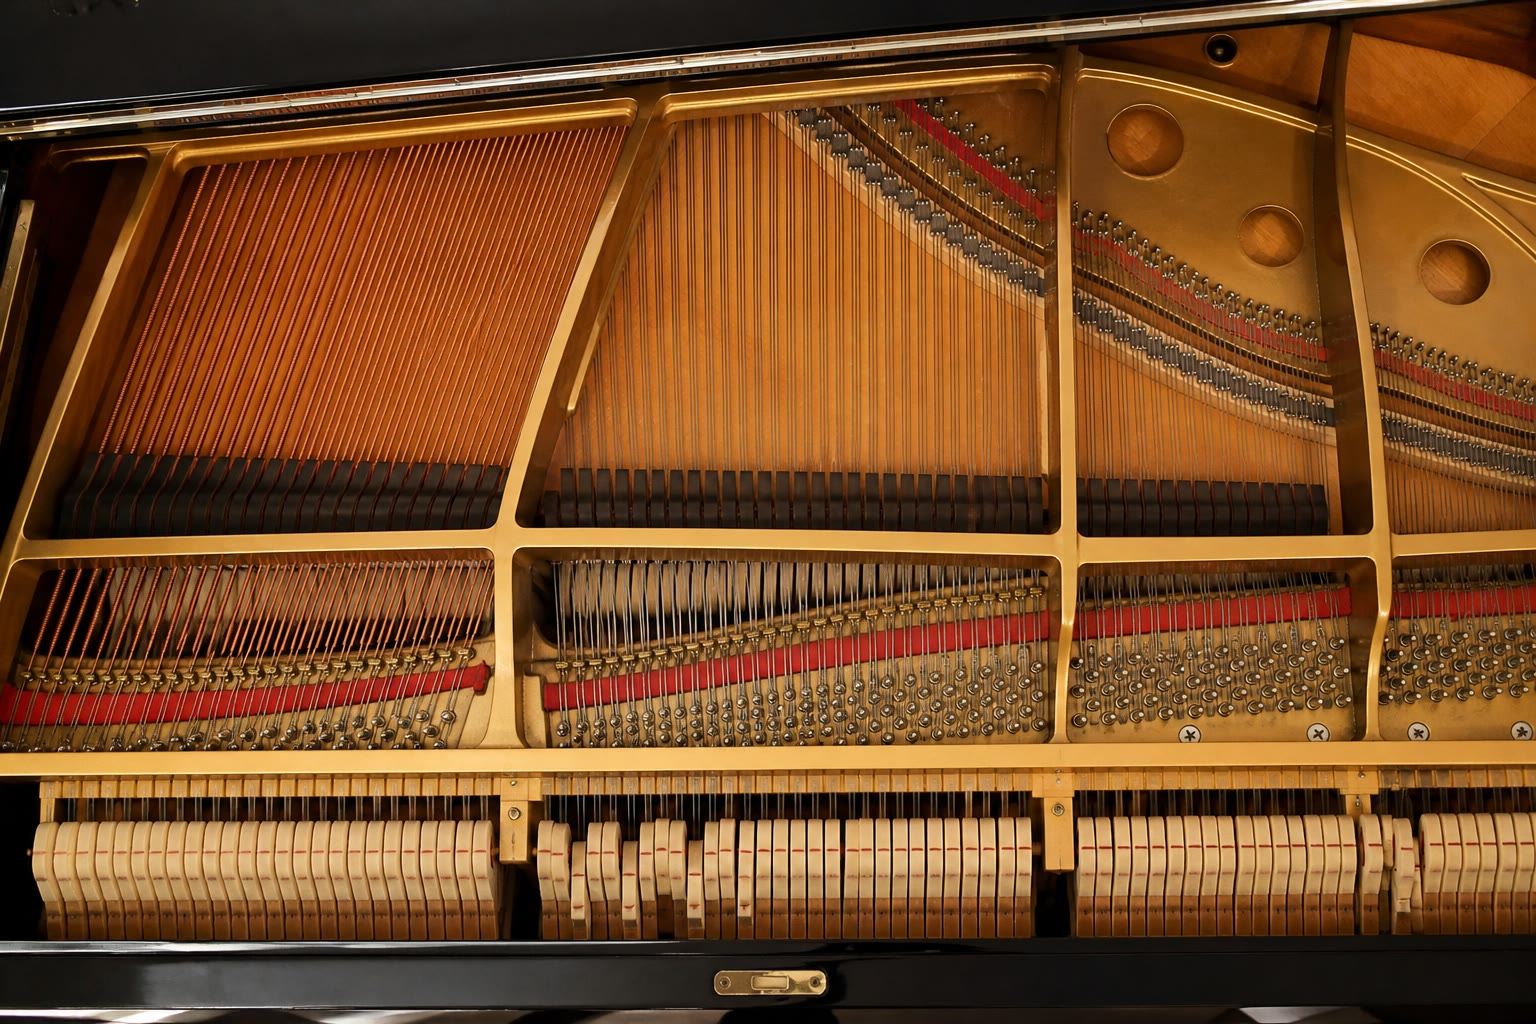
\includegraphics[width=0.58\linewidth]{images/book4/ai/b4-06-grand-piano-strings.jpg}

{\small Por dentro de um piano de cauda: cerca de duzentas cordas de aço de comprimento e espessura graduados, cada uma afinada por sua tração a um fundamental $c/2L$; as cordas graves são encapadas com cobre para ganhar massa.}
\end{omfigure}

\section{Problema: O piano, do martelo ao tampo harmônico}

\begin{problem}[{Problema de fim de semana --- uma corda de piano desmontada: sua
tração e sua rigidez, o golpe do martelo e os harmônicos que ele cria,
o cavalete que escoa sua energia para o tampo harmônico, e um trilho que
carrega a mesma equação}]
\label{pb:b2:waves-on-strings:1}

\medskip
\noindent\textbf{Parte I --- A corda.}
A corda lá$_4$ de um piano (\qty{440}{Hz}): aço, $E = \qty{200}{GPa}$, $\rho =
\qty{7800}{kg/m^3}$, diâmetro $d = \qty{1.0}{mm}$, comprimento vibrante $L =
\qty{38}{cm}$. Cada nota acima do registro grave tem três cordas dessas; o piano
tem $230$ cordas.
\begin{enumerate}
  \item Massa linear, celeridade das ondas e tração da corda.
  \item Tensão de tração no fio; o fio rompe a \qty{2.0}{GPa}: a
        margem de segurança, e por que a última volta do afinador é a
        perigosa.
  \item Estime a tração total sobre a placa, supondo todas as cordas
        na mesma tração.
  \item A corda mais grave (lá$_0$, \qty{27.5}{Hz}) tem \qty{1.9}{m}; se ela
        fosse um fio de aço liso à mesma tração, de que $\mu$ e de
        que diâmetro precisaria? Ela é, na verdade, um núcleo de aço encapado com
        cobre: explique.
  \item Modos da corda lá$_4$: frequências dos oito primeiros
        harmônicos; quais deles ficam num intervalo consonante com o
        fundamental (oitava, quinta, quarta, terça maior) e quais
        não?
  \item A corda vibra em seu fundamental com amplitude de
        \qty{0.50}{mm} no ventre: energia armazenada (a energia de um
        modo vale $\tfrac14\mu L\omega^2A^2$).
  \item Escreva o fundamental como soma de duas ondas progressivas; dê
        a amplitude de cada uma e a potência média que cada uma transporta.
\end{enumerate}

\medskip
\noindent\textbf{Parte II --- O martelo.}
O martelo golpeia a corda em $x_0 = L/8$, dando-lhe, em $t = 0$, uma
velocidade $v_0$ num trecho curto de largura $w$ em torno de $x_0$ e nenhum
deslocamento.
\begin{enumerate}[resume]
  \item Escreva a solução geral $y = \sum_nB_n\sin(n\pi x/L)\sin(\omega_nt)$
        e mostre, usando a ortogonalidade dos senos, que $B_n =
        \dfrac{2}{L\omega_n}\int_0^L\dot y(x, 0)\sin\dfrac{n\pi x}L\,\dd x$.
  \item Para um golpe estreito ($w \ll L/n$), mostre que $B_n \approx \dfrac{2v_0w}
        {L\omega_n}\sin\dfrac{n\pi x_0}{L}$.
  \item Que harmônicos estão ausentes para $x_0 = L/8$? Por que os
        fabricantes de piano golpeiam entre $L/7$ e $L/8$ (veja a questão 5)?
  \item Descreva o movimento na imagem das ondas progressivas: o que
        parte do ponto golpeado, o que acontece nas extremidades e ao cabo
        de que tempo o estado inicial se repete.
  \item Uma corda real é ligeiramente rígida: seus modos são $f_n = nf_1
        \sqrt{1 + Bn^2}$ com $B = \pi^3Ed^4/(64TL^2)$ (admitido). Calcule
        $B$ e o quanto o oitavo harmônico fica agudo, em por cento e
        em cents (\qty{1}{cent} = uma razão de frequências $2^{1/1200}$).
  \item Por que os afinadores de piano "esticam" as oitavas (afinam as notas agudas
        um pouco mais altas)?
\end{enumerate}

\medskip
\noindent\textbf{Parte III --- O cavalete e o tampo harmônico.}
A corda passa por um cavalete colado ao tampo harmônico; o tampo
comporta-se, no cavalete, como uma corda de impedância $Z_b = \qty{2000}{kg/s}$.
\begin{enumerate}[resume]
  \item Impedância $Z_s$ da corda; coeficiente de reflexão em amplitude
        no cavalete.
  \item Fração da energia da onda transmitida ao tampo a
        cada reflexão.
  \item Número de reflexões por segundo no cavalete; deduza a constante
        de tempo do decaimento da energia e o tempo para o som cair
        \qty{60}{dB} (um fator $10^6$ em energia).
  \item Potência que escoa para o tampo logo após o golpe da
        questão 6; compare com a potência de uma conversa tranquila,
        cerca de \qty{1e-5}{W} de som.
  \item Por que uma corda sozinha é quase inaudível, e o que o
        tampo faz a respeito? (Pense na impedância do ar,
        $\rho c \approx \qty{400}{kg.m^{-2}.s^{-1}}$, vista através de uma superfície
        pequena contra uma grande.)
  \item Com o abafador levantado, a corda lá$_3$ (\qty{220}{Hz}) começa a
        soar quando se toca lá$_4$: por quê?
  \item Um fabricante quer uma sustentação mais longa: $Z_b$ deve ser aumentada ou
        diminuída, e o que se perde com isso?
\end{enumerate}

\medskip
\noindent\textbf{Parte IV --- O trilho.}
Um trilho de aço ($E = \qty{200}{GPa}$, $\rho = \qty{7800}{kg/m^3}$, seção
\qty{70}{cm^2}).
\begin{enumerate}[resume]
  \item Celeridade das ondas de compressão; tempo para o som de um trem
        percorrer \qty{5}{km} pelo trilho e pelo ar.
  \item Uma martelada envia um pulso de compressão por um trecho de trilho de
        \qty{25}{m} com extremidade livre: tempo do eco; o eco é uma
        compressão ou uma rarefação?
  \item Uma sonda ultrassônica de \qty{2}{MHz} procura trincas: comprimento de onda no
        aço; coeficiente de reflexão em amplitude numa trinca aço--ar
        (impedância do ar $\qty{400}{kg.m^{-2}.s^{-1}}$); por que uma trinca
        fina é vista tão bem.
  \item Terremotos: na rocha, as ondas de compressão (P) viajam a
        \qty{6.0}{km/s} e as de cisalhamento (S) a \qty{3.5}{km/s}. Uma estação
        registra a onda S \qty{20}{s} depois da onda P: distância até a
        fonte.
  \item Numa tabela, reúna as cinco celeridades de onda deste problema
        (corda, trilho, P na rocha, S na rocha, ar) com a rigidez e a
        inércia que fixam cada uma.
\end{enumerate}
\end{problem}
